\documentclass[tikz,border=2mm]{standalone}
\usepackage{tikz}
\usetikzlibrary{trees, arrows}

\begin{document}

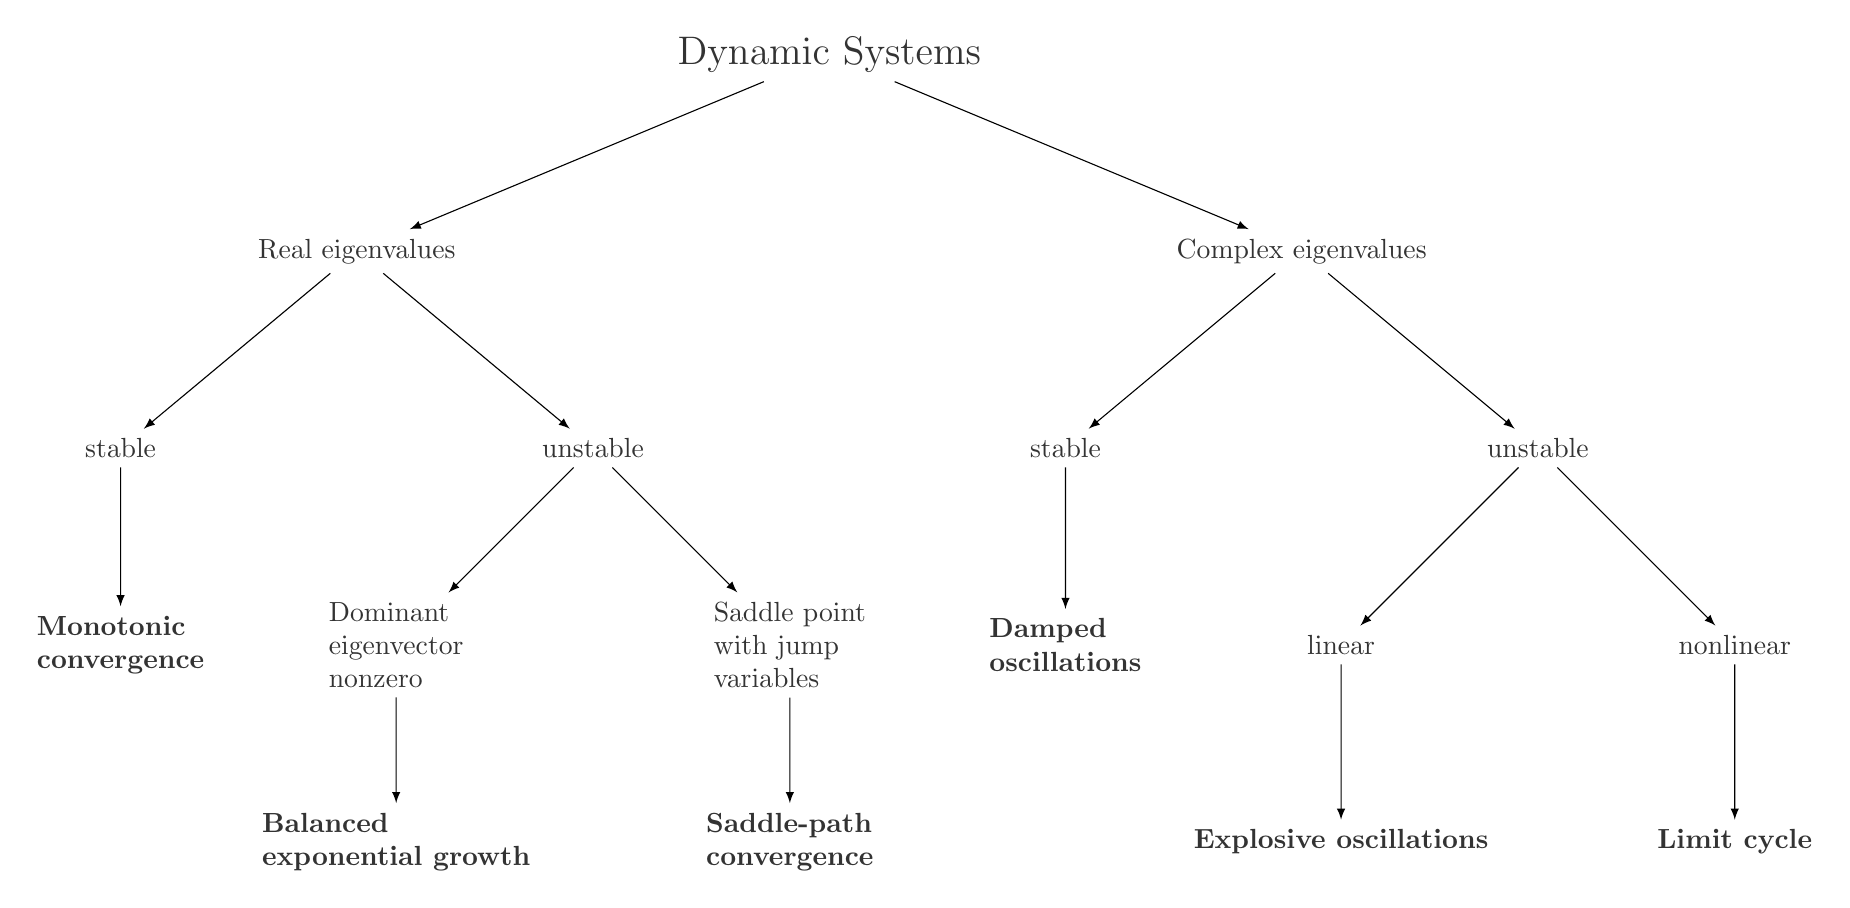
\begin{tikzpicture}[level distance=2.5cm,
level 1/.style={sibling distance=12cm},
level 2/.style={sibling distance=6cm},
level 3/.style={sibling distance=5cm},
every node/.style = {shape=rectangle, align=center, color=black!80},
edge from parent/.style={draw,-latex}]
%
\node [] {{\Large Dynamic Systems}}
	child { node[] (real) {Real eigenvalues}
		child { node[] (stable_real) {stable}
			child { node[align=left] {\textbf{Monotonic} \\ \textbf{convergence}}} }
		child { node[] (unstable_real) {unstable}
			child { node[align=left] (dominantnonzero) {Dominant \\ eigenvector \\ nonzero}
				child { node[align=left] {\textbf{Balanced} \\ \textbf{exponential growth}}} }
			child { node[align=left] (saddle) {Saddle point \\ with jump \\ variables}
				child { node[align=left] {\textbf{Saddle-path} \\ \textbf{convergence}}} } }
	}
	child { node[] (complex) {Complex eigenvalues}
		child { node[] {stable}
			child { node[align=left] (damped) {\textbf{Damped} \\ \textbf{oscillations}}} }
		child { node[] (unstable) {unstable}
			child { node[] (linear) {linear}
				child { node (explosive) {\textbf{Explosive oscillations}} } }
			child { node[] (nonlinear1) {nonlinear}
				child { node (limitcycle) {\textbf{Limit cycle}} } } }
	}
;
\end{tikzpicture}

\end{document}
